\documentclass{article}

\usepackage{ross}
\newcommand{\labelthis}[1]{\addtocounter{equation}{1}\tag{\theequation}\label{#1}}
\usepackage{tikz}
\fancyhdr

\begin{document}
\makeheading{Elliptic Spectral Curve}
\section{Elliptic Integrals}
Elliptic integrals are ones that arise as the integrals of differentials on elliptic curves (curves of genus one). There are several sets of standard elliptic integrals, with the idea being that every elliptic integral can be reduced to a combination of the standard ones in a particular set. The most prevalent set, the Jacobi elliptic integrals, is used here. Note however that there are several variations in nototation about these integrals; the main difference is the use of the modulus $k$ versus the parameter $m = k^2$. We will us the former. There are three standard integrals, and they come in {\it incomplete} and {\it complete} varities. The complete elliptic integral of first kind is denoted $K$ and is defined as
\[
K = K(k) = \int_0^1 \frac{dt}{\sqrt{(1-t^2)(1-k^2 t^2)}} .
\]
The complete elliptic integral of second kind is denoted $E$ and is defined as
\[
E = E(k) = \int_0^1 \sqrt{\frac{1-k^2 t^2}{1-t^2}} \;dt = \int_0^1 \frac{1-k^2 t^2}{\sqrt{(1-t^2)(1-k^2 t^2)}}\;dt .
\]
We will not have need of the others. Elliptic integrals of the first kind correspond to holomorphic forms, so one can see from the form above that the curve is given by the equation
\[
y^2 = (1-t^2)(1-k^2 t^2).
\]
This highly symmetric form is known as {\it Lagrange form}. By M\"obius transformation (or by Landen's transformations), when $k$ is real one can arrange for $0< k < 1$, where the extremes of $k=0$ and $k=1$ reduces things to regular circle trigonomtry. The period of this curve around the branch points $-1$ and $1$ is obiviously related to the definitions above. For example, this period of the holomorphic differential is precisely $4K$, which earns $K$ the nickname of `quarter-period'.

\begin{center}
% Sketch output, version 0.3 (build 7d, Tue Sep 23 14:56:38 2014)
% Output language: PGF/TikZ,LaTeX
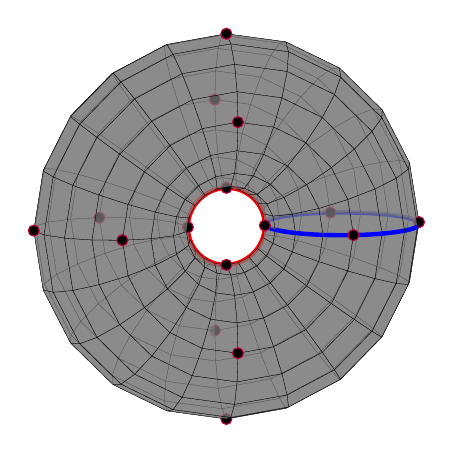
\begin{tikzpicture}[line join=round]
\filldraw[draw=black,ultra thin,fill=gray,fill opacity=0.7](1.643,-1.129)--(1.354,-.917)--(.947,-1.334)--(1.165,-1.618)--cycle;
\filldraw[draw=black,ultra thin,fill=gray,fill opacity=0.7](1.354,-.917)--(1.04,-.693)--(.716,-1.025)--(.947,-1.334)--cycle;
\filldraw[draw=black,ultra thin,fill=gray,fill opacity=0.7](1.95,-.521)--(1.616,-.398)--(1.354,-.917)--(1.643,-1.129)--cycle;
\filldraw[draw=black,ultra thin,fill=gray,fill opacity=0.7](1.616,-.398)--(1.249,-.279)--(1.04,-.693)--(1.354,-.917)--cycle;
\filldraw[draw=black,ultra thin,fill=gray,fill opacity=0.7](.947,-1.334)--(.716,-1.025)--(.307,-1.242)--(.434,-1.607)--cycle;
\filldraw[draw=black,ultra thin,fill=gray,fill opacity=0.7](1.165,-1.618)--(.947,-1.334)--(.434,-1.607)--(.563,-1.938)--cycle;
\filldraw[draw=black,ultra thin,fill=gray,fill opacity=0.7](1.249,-.279)--(.904,-.182)--(.749,-.491)--(1.04,-.693)--cycle;
\filldraw[draw=black,ultra thin,fill=gray,fill opacity=0.7](1.04,-.693)--(.749,-.491)--(.507,-.738)--(.716,-1.025)--cycle;
\filldraw[draw=black,ultra thin,fill=gray,fill opacity=0.7](.716,-1.025)--(.507,-.738)--(.202,-.9)--(.307,-1.242)--cycle;
\filldraw[draw=black,ultra thin,fill=gray,fill opacity=0.7](.307,-1.242)--(.202,-.9)--(-.136,-.961)--(-.147,-1.324)--cycle;
\filldraw[draw=black,ultra thin,fill=gray,fill opacity=0.7](.434,-1.607)--(.307,-1.242)--(-.147,-1.324)--(-.136,-1.71)--cycle;
\filldraw[draw=black,ultra thin,fill=gray,fill opacity=0.7](1.706,.173)--(1.321,.176)--(1.249,-.279)--(1.616,-.398)--cycle;
\filldraw[draw=black,ultra thin,fill=gray,fill opacity=0.7](1.321,.176)--(.957,.157)--(.904,-.182)--(1.249,-.279)--cycle;
\filldraw[draw=black,ultra thin,fill=gray,fill opacity=0.7](2.055,.149)--(1.706,.173)--(1.616,-.398)--(1.95,-.521)--cycle;
\filldraw[draw=black,ultra thin,fill=gray,fill opacity=0.7](.563,-1.938)--(.434,-1.607)--(-.136,-1.71)--(-.104,-2.058)--cycle;
\draw[draw=blue,ultra thick](1.7,.173)--(1.63,.175)--(1.527,.177)--(1.424,.177)--(1.321,.176);
\draw[draw=blue,ultra thick](1.321,.176)--(1.219,.173)--(1.12,.168)--(1.026,.162)--(.963,.157);
\filldraw[draw=black,ultra thin,fill=gray,fill opacity=0.7](1.616,.74)--(1.249,.628)--(1.321,.176)--(1.706,.173)--cycle;
\filldraw[draw=black,ultra thin,fill=gray,fill opacity=0.7](1.249,.628)--(.904,.493)--(.957,.157)--(1.321,.176)--cycle;
\filldraw[draw=purple](-.147,-1.324) circle (2pt);
\filldraw[draw=black,ultra thin,fill=gray,fill opacity=0.7](-.136,-1.71)--(-.147,-1.324)--(-.6,-1.262)--(-.705,-1.632)--cycle;
\filldraw[draw=black,ultra thin,fill=gray,fill opacity=0.7](-.147,-1.324)--(-.136,-.961)--(-.473,-.915)--(-.6,-1.262)--cycle;
\filldraw[draw=purple](1.321,.176) circle (2pt);
\draw[draw=blue,ultra thick](1.71,.173)--(1.7,.173);
\draw[draw=blue,ultra thick](2.049,.149)--(2.013,.153)--(1.924,.161)--(1.829,.167)--(1.731,.172)--(1.71,.173);
\filldraw[draw=black,ultra thin,fill=gray,fill opacity=0.7](1.95,.814)--(1.616,.74)--(1.706,.173)--(2.055,.149)--cycle;
\filldraw[draw=black,ultra thin,fill=gray,fill opacity=0.7](-.104,-2.058)--(-.136,-1.71)--(-.705,-1.632)--(-.771,-1.967)--cycle;
\filldraw[draw=black,ultra thin,fill=gray,fill opacity=0.7](1.862,-1.297)--(1.643,-1.129)--(1.165,-1.618)--(1.338,-1.833)--cycle;
\filldraw[draw=black,ultra thin,fill=gray,fill opacity=0.7](1.338,-1.833)--(1.165,-1.618)--(.563,-1.938)--(.677,-2.185)--cycle;
\filldraw[draw=black,ultra thin,fill=gray,fill opacity=0.7](2.199,-.628)--(1.95,-.521)--(1.643,-1.129)--(1.862,-1.297)--cycle;
\filldraw[draw=black,ultra thin,fill=gray,fill opacity=0.7](.904,-.182)--(.634,-.122)--(.524,-.341)--(.749,-.491)--cycle;
\filldraw[draw=black,ultra thin,fill=gray,fill opacity=0.7](.749,-.491)--(.524,-.341)--(.352,-.516)--(.507,-.738)--cycle;
\filldraw[draw=black,ultra thin,fill=gray,fill opacity=0.7](.507,-.738)--(.352,-.516)--(.136,-.631)--(.202,-.9)--cycle;
\filldraw[draw=black,ultra thin,fill=gray,fill opacity=0.7](-.6,-1.262)--(-.473,-.915)--(-.778,-.766)--(-1.009,-1.063)--cycle;
\filldraw[draw=black,ultra thin,fill=gray,fill opacity=0.7](-.705,-1.632)--(-.6,-1.262)--(-1.009,-1.063)--(-1.218,-1.382)--cycle;
\filldraw[draw=black,ultra thin,fill=gray,fill opacity=0.7](1.04,1.032)--(.749,.795)--(.904,.493)--(1.249,.628)--cycle;
\filldraw[draw=black,ultra thin,fill=gray,fill opacity=0.7](1.354,1.248)--(1.04,1.032)--(1.249,.628)--(1.616,.74)--cycle;
\filldraw[draw=black,ultra thin,fill=gray,fill opacity=0.7](.957,.157)--(.672,.119)--(.634,-.122)--(.904,-.182)--cycle;
\filldraw[draw=black,ultra thin,fill=gray,fill opacity=0.7](.202,-.9)--(.136,-.631)--(-.104,-.674)--(-.136,-.961)--cycle;
\filldraw[draw=black,ultra thin,fill=gray,fill opacity=0.7](.677,-2.185)--(.563,-1.938)--(-.104,-2.058)--(-.056,-2.317)--cycle;
\filldraw[draw=black,ultra thin,fill=gray,fill opacity=0.7](2.315,.107)--(2.055,.149)--(1.95,-.521)--(2.199,-.628)--cycle;
\filldraw[draw=black,ultra thin,fill=gray,fill opacity=0.7](1.643,1.409)--(1.354,1.248)--(1.616,.74)--(1.95,.814)--cycle;
\filldraw[draw=black,ultra thin,fill=gray,fill opacity=0.7](-.771,-1.967)--(-.705,-1.632)--(-1.218,-1.382)--(-1.373,-1.674)--cycle;
\draw[draw=blue,ultra thick](.963,.157)--(.954,.156);
\draw[draw=blue,ultra thick](.954,.156)--(.935,.155)--(.851,.146)--(.774,.136)--(.704,.125)--(.677,.119);
\filldraw[draw=black,ultra thin,fill=gray,fill opacity=0.7](.904,.493)--(.634,.357)--(.672,.119)--(.957,.157)--cycle;
\filldraw[draw=black,ultra thin,fill=gray,fill opacity=0.7](-.136,-.961)--(-.104,-.674)--(-.343,-.642)--(-.473,-.915)--cycle;
\filldraw[draw=black,ultra thin,fill=gray,fill opacity=0.7](.716,1.35)--(.507,1.031)--(.749,.795)--(1.04,1.032)--cycle;
\filldraw[draw=black,ultra thin,fill=gray,fill opacity=0.7](.947,1.647)--(.716,1.35)--(1.04,1.032)--(1.354,1.248)--cycle;
\filldraw[draw=black,ultra thin,fill=gray,fill opacity=0.7](-1.218,-1.382)--(-1.009,-1.063)--(-1.334,-.745)--(-1.626,-.983)--cycle;
\filldraw[draw=black,ultra thin,fill=gray,fill opacity=0.7](-1.009,-1.063)--(-.778,-.766)--(-1.02,-.529)--(-1.334,-.745)--cycle;
\draw[draw=blue,ultra thick](2.06,.148)--(2.049,.149);
\draw[draw=blue,ultra thick](2.312,.108)--(2.301,.11)--(2.241,.123)--(2.173,.134)--(2.096,.144)--(2.06,.148);
\filldraw[draw=black,ultra thin,fill=gray,fill opacity=0.7](2.199,.837)--(1.95,.814)--(2.055,.149)--(2.315,.107)--cycle;
\filldraw[draw=black,ultra thin,fill=gray,fill opacity=0.7](-.056,-2.317)--(-.104,-2.058)--(-.771,-1.967)--(-.789,-2.217)--cycle;
\filldraw[draw=black,ultra thin,fill=gray,fill opacity=0.7](.749,.795)--(.524,.571)--(.634,.357)--(.904,.493)--cycle;
\filldraw[draw=black,ultra thin,fill=gray,fill opacity=0.7](-.473,-.915)--(-.343,-.642)--(-.56,-.536)--(-.778,-.766)--cycle;
\filldraw[draw=black,ultra thin,fill=gray,fill opacity=0.7](1.165,1.877)--(.947,1.647)--(1.354,1.248)--(1.643,1.409)--cycle;
\filldraw[draw=black,ultra thin,fill=gray,fill opacity=0.7](-1.373,-1.674)--(-1.218,-1.382)--(-1.626,-.983)--(-1.85,-1.206)--cycle;
\filldraw[draw=black,ultra thin,fill=gray,fill opacity=0.7](-.778,-.766)--(-.56,-.536)--(-.731,-.368)--(-1.02,-.529)--cycle;
\filldraw[draw=black,ultra thin,fill=gray,fill opacity=0.7](.507,1.031)--(.352,.739)--(.524,.571)--(.749,.795)--cycle;
\filldraw[draw=black,ultra thin,fill=gray,fill opacity=0.7](.434,1.897)--(.307,1.549)--(.716,1.35)--(.947,1.647)--cycle;
\filldraw[draw=black,ultra thin,fill=gray,fill opacity=0.7](.307,1.549)--(.202,1.18)--(.507,1.031)--(.716,1.35)--cycle;
\filldraw[draw=black,ultra thin,fill=gray,fill opacity=0.7](-1.626,-.983)--(-1.334,-.745)--(-1.542,-.341)--(-1.887,-.475)--cycle;
\filldraw[draw=black,ultra thin,fill=gray,fill opacity=0.7](-1.334,-.745)--(-1.02,-.529)--(-1.175,-.228)--(-1.542,-.341)--cycle;
\filldraw[draw=black,ultra thin,fill=gray,fill opacity=0.7](1.862,1.491)--(1.643,1.409)--(1.95,.814)--(2.199,.837)--cycle;
\filldraw[draw=black,ultra thin,fill=gray,fill opacity=0.7](-.789,-2.217)--(-.771,-1.967)--(-1.373,-1.674)--(-1.45,-1.894)--cycle;
\filldraw[draw=black,ultra thin,fill=gray,fill opacity=0.7](1.437,-1.947)--(1.338,-1.833)--(.677,-2.185)--(.756,-2.31)--cycle;
\filldraw[draw=black,ultra thin,fill=gray,fill opacity=0.7](1.979,-1.394)--(1.862,-1.297)--(1.338,-1.833)--(1.437,-1.947)--cycle;
\filldraw[draw=black,ultra thin,fill=gray,fill opacity=0.7](2.326,-.705)--(2.199,-.628)--(1.862,-1.297)--(1.979,-1.394)--cycle;
\filldraw[draw=black,ultra thin,fill=gray,fill opacity=0.7](-1.02,-.529)--(-.731,-.368)--(-.841,-.154)--(-1.175,-.228)--cycle;
\filldraw[draw=black,ultra thin,fill=gray,fill opacity=0.7](.202,1.18)--(.136,.845)--(.352,.739)--(.507,1.031)--cycle;
\filldraw[draw=black,ultra thin,fill=gray,fill opacity=0.7](.352,-.516)--(.275,-.394)--(.118,-.477)--(.136,-.631)--cycle;
\filldraw[draw=black,ultra thin,fill=gray,fill opacity=0.7](.524,-.341)--(.4,-.266)--(.275,-.394)--(.352,-.516)--cycle;
\filldraw[draw=black,ultra thin,fill=gray,fill opacity=0.7](.634,-.122)--(.48,-.107)--(.4,-.266)--(.524,-.341)--cycle;
\filldraw[draw=black,ultra thin,fill=gray,fill opacity=0.7](.563,2.17)--(.434,1.897)--(.947,1.647)--(1.165,1.877)--cycle;
\filldraw[draw=black,ultra thin,fill=gray,fill opacity=0.7](-1.85,-1.206)--(-1.626,-.983)--(-1.887,-.475)--(-2.157,-.611)--cycle;
\filldraw[draw=black,ultra thin,fill=gray,fill opacity=0.7](.136,-.631)--(.118,-.477)--(-.056,-.509)--(-.104,-.674)--cycle;
\filldraw[draw=black,ultra thin,fill=gray,fill opacity=0.7](.672,.119)--(.507,.067)--(.48,-.107)--(.634,-.122)--cycle;
\filldraw[draw=black,ultra thin,fill=gray,fill opacity=0.7](-1.542,-.341)--(-1.175,-.228)--(-1.229,.109)--(-1.614,.111)--cycle;
\filldraw[draw=black,ultra thin,fill=gray,fill opacity=0.7](-1.887,-.475)--(-1.542,-.341)--(-1.614,.111)--(-1.977,.092)--cycle;
\filldraw[draw=black,ultra thin,fill=gray,fill opacity=0.7](-.147,1.611)--(-.136,1.226)--(.202,1.18)--(.307,1.549)--cycle;
\filldraw[draw=black,ultra thin,fill=gray,fill opacity=0.7](-.136,1.975)--(-.147,1.611)--(.307,1.549)--(.434,1.897)--cycle;
\filldraw[draw=black,ultra thin,fill=gray,fill opacity=0.7](.756,-2.31)--(.677,-2.185)--(-.056,-2.317)--(0,-2.446)--cycle;
\filldraw[draw=black,ultra thin,fill=gray,fill opacity=0.7](2.446,.054)--(2.315,.107)--(2.199,-.628)--(2.326,-.705)--cycle;
\draw[draw=blue,ultra thick](.677,.119)--(.669,.118);
\filldraw[draw=black,ultra thin,fill=gray,fill opacity=0.7](-.104,-.674)--(-.056,-.509)--(-.23,-.485)--(-.343,-.642)--cycle;
\draw[draw=blue,ultra thick](.669,.118)--(.642,.112)--(.59,.099)--(.547,.085)--(.514,.071)--(.509,.068);
\filldraw[draw=black,ultra thin,fill=gray,fill opacity=0.7](.634,.357)--(.48,.241)--(.507,.067)--(.672,.119)--cycle;
\filldraw[draw=black,ultra thin,fill=gray,fill opacity=0.7](-1.175,-.228)--(-.841,-.154)--(-.879,.084)--(-1.229,.109)--cycle;
\filldraw[draw=black,ultra thin,fill=gray,fill opacity=0.7](-.136,1.226)--(-.104,.877)--(.136,.845)--(.202,1.18)--cycle;
\filldraw[draw=black,ultra thin,fill=gray,fill opacity=0.7](.524,.571)--(.4,.396)--(.48,.241)--(.634,.357)--cycle;
\filldraw[draw=black,ultra thin,fill=gray,fill opacity=0.7](-.343,-.642)--(-.23,-.485)--(-.387,-.408)--(-.56,-.536)--cycle;
\filldraw[draw=black,ultra thin,fill=gray,fill opacity=0.7](-1.45,-1.894)--(-1.373,-1.674)--(-1.85,-1.206)--(-1.974,-1.381)--cycle;
\filldraw[draw=black,ultra thin,fill=gray,fill opacity=0.7](1.338,2.004)--(1.165,1.877)--(1.643,1.409)--(1.862,1.491)--cycle;
\filldraw[draw=black,ultra thin,fill=gray,fill opacity=0.7](-.705,1.872)--(-.6,1.529)--(-.147,1.611)--(-.136,1.975)--cycle;
\filldraw[draw=black,ultra thin,fill=gray,fill opacity=0.7](-.6,1.529)--(-.473,1.165)--(-.136,1.226)--(-.147,1.611)--cycle;
\filldraw[draw=black,ultra thin,fill=gray,fill opacity=0.7](-1.977,.092)--(-1.614,.111)--(-1.542,.566)--(-1.887,.663)--cycle;
\filldraw[draw=black,ultra thin,fill=gray,fill opacity=0.7](-1.614,.111)--(-1.229,.109)--(-1.175,.448)--(-1.542,.566)--cycle;
\filldraw[draw=purple](-.147,1.611) circle (2pt);
\filldraw[draw=purple](-1.614,.111) circle (2pt);
\filldraw[draw=black,ultra thin,fill=gray,fill opacity=0.7](-1.229,.109)--(-.879,.084)--(-.841,.325)--(-1.175,.448)--cycle;
\filldraw[draw=black,ultra thin,fill=gray,fill opacity=0.7](-.473,1.165)--(-.343,.834)--(-.104,.877)--(-.136,1.226)--cycle;
\draw[draw=blue,ultra thick](2.317,.106)--(2.312,.108);
\draw[draw=blue,ultra thick](2.446,.054)--(2.425,.069)--(2.394,.083)--(2.352,.097)--(2.317,.106);
\filldraw[draw=black,ultra thin,fill=gray,fill opacity=0.7](2.326,.807)--(2.199,.837)--(2.315,.107)--(2.446,.054)--cycle;
\filldraw[draw=black,ultra thin,fill=gray,fill opacity=0.7](0,-2.446)--(-.056,-2.317)--(-.789,-2.217)--(-.756,-2.343)--cycle;
\filldraw[draw=black,ultra thin,fill=gray,fill opacity=0.7](-.104,2.261)--(-.136,1.975)--(.434,1.897)--(.563,2.17)--cycle;
\filldraw[draw=black,ultra thin,fill=gray,fill opacity=0.7](-2.157,-.611)--(-1.887,-.475)--(-1.977,.092)--(-2.263,.054)--cycle;
\filldraw[draw=black,ultra thin,fill=gray,fill opacity=0.7](-.56,-.536)--(-.387,-.408)--(-.512,-.286)--(-.731,-.368)--cycle;
\filldraw[draw=black,ultra thin,fill=gray,fill opacity=0.7](.352,.739)--(.275,.518)--(.4,.396)--(.524,.571)--cycle;
\filldraw[draw=black,ultra thin,fill=gray,fill opacity=0.7](-1.887,.663)--(-1.542,.566)--(-1.334,.98)--(-1.626,1.183)--cycle;
\filldraw[draw=black,ultra thin,fill=gray,fill opacity=0.7](-1.542,.566)--(-1.175,.448)--(-1.02,.756)--(-1.334,.98)--cycle;
\filldraw[draw=black,ultra thin,fill=gray,fill opacity=0.7](-1.009,1.312)--(-.778,1.003)--(-.473,1.165)--(-.6,1.529)--cycle;
\filldraw[draw=black,ultra thin,fill=gray,fill opacity=0.7](-1.218,1.599)--(-1.009,1.312)--(-.6,1.529)--(-.705,1.872)--cycle;
\filldraw[draw=black,ultra thin,fill=gray,fill opacity=0.7](-.778,1.003)--(-.56,.719)--(-.343,.834)--(-.473,1.165)--cycle;
\filldraw[draw=black,ultra thin,fill=gray,fill opacity=0.7](-1.175,.448)--(-.841,.325)--(-.731,.544)--(-1.02,.756)--cycle;
\filldraw[draw=black,ultra thin,fill=gray,fill opacity=0.7](-1.02,.756)--(-.731,.544)--(-.56,.719)--(-.778,1.003)--cycle;
\filldraw[draw=black,ultra thin,fill=gray,fill opacity=0.7](-1.334,.98)--(-1.02,.756)--(-.778,1.003)--(-1.009,1.312)--cycle;
\filldraw[draw=black,ultra thin,fill=gray,fill opacity=0.7](-1.626,1.183)--(-1.334,.98)--(-1.009,1.312)--(-1.218,1.599)--cycle;
\filldraw[draw=black,ultra thin,fill=gray,fill opacity=0.7](.136,.845)--(.118,.595)--(.275,.518)--(.352,.739)--cycle;
\filldraw[draw=black,ultra thin,fill=gray,fill opacity=0.7](-.731,-.368)--(-.512,-.286)--(-.592,-.131)--(-.841,-.154)--cycle;
\filldraw[draw=black,ultra thin,fill=gray,fill opacity=0.7](-.771,2.141)--(-.705,1.872)--(-.136,1.975)--(-.104,2.261)--cycle;
\filldraw[draw=black,ultra thin,fill=gray,fill opacity=0.7](-2.263,.054)--(-1.977,.092)--(-1.887,.663)--(-2.157,.724)--cycle;
\filldraw[draw=black,ultra thin,fill=gray,fill opacity=0.7](.677,2.327)--(.563,2.17)--(1.165,1.877)--(1.338,2.004)--cycle;
\filldraw[draw=black,ultra thin,fill=gray,fill opacity=0.7](-1.974,-1.381)--(-1.85,-1.206)--(-2.157,-.611)--(-2.311,-.728)--cycle;
\filldraw[draw=black,ultra thin,fill=gray,fill opacity=0.7](-.841,-.154)--(-.592,-.131)--(-.62,.043)--(-.879,.084)--cycle;
\filldraw[draw=black,ultra thin,fill=gray,fill opacity=0.7](-.104,.877)--(-.056,.619)--(.118,.595)--(.136,.845)--cycle;
\filldraw[draw=black,ultra thin,fill=gray,fill opacity=0.7](1.979,1.481)--(1.862,1.491)--(2.199,.837)--(2.326,.807)--cycle;
\filldraw[draw=black,ultra thin,fill=gray,fill opacity=0.7](-.756,-2.343)--(-.789,-2.217)--(-1.45,-1.894)--(-1.437,-2.011)--cycle;
\filldraw[draw=black,ultra thin,fill=gray,fill opacity=0.7](-.879,.084)--(-.62,.043)--(-.592,.217)--(-.841,.325)--cycle;
\filldraw[draw=black,ultra thin,fill=gray,fill opacity=0.7](-.343,.834)--(-.23,.587)--(-.056,.619)--(-.104,.877)--cycle;
\filldraw[draw=black,ultra thin,fill=gray,fill opacity=0.7](-1.373,1.821)--(-1.218,1.599)--(-.705,1.872)--(-.771,2.141)--cycle;
\filldraw[draw=black,ultra thin,fill=gray,fill opacity=0.7](-2.157,.724)--(-1.887,.663)--(-1.626,1.183)--(-1.85,1.332)--cycle;
\filldraw[draw=black,ultra thin,fill=gray,fill opacity=0.7](-.841,.325)--(-.592,.217)--(-.512,.376)--(-.731,.544)--cycle;
\filldraw[draw=black,ultra thin,fill=gray,fill opacity=0.7](-.56,.719)--(-.387,.504)--(-.23,.587)--(-.343,.834)--cycle;
\filldraw[draw=black,ultra thin,fill=gray,fill opacity=0.7](-.731,.544)--(-.512,.376)--(-.387,.504)--(-.56,.719)--cycle;
\filldraw[draw=black,ultra thin,fill=gray,fill opacity=0.7](-1.85,1.332)--(-1.626,1.183)--(-1.218,1.599)--(-1.373,1.821)--cycle;
\filldraw[draw=black,ultra thin,fill=gray,fill opacity=0.7](1.45,-1.943)--(1.437,-1.947)--(.756,-2.31)--(.789,-2.294)--cycle;
\filldraw[draw=black,ultra thin,fill=gray,fill opacity=0.7](1.974,-1.407)--(1.979,-1.394)--(1.437,-1.947)--(1.45,-1.943)--cycle;
\filldraw[draw=black,ultra thin,fill=gray,fill opacity=0.7](2.311,-.738)--(2.326,-.705)--(1.979,-1.394)--(1.974,-1.407)--cycle;
\filldraw[draw=black,ultra thin,fill=gray,fill opacity=0.7](.275,-.394)--(.287,-.389)--(.151,-.462)--(.118,-.477)--cycle;
\filldraw[draw=black,ultra thin,fill=gray,fill opacity=0.7](.4,-.266)--(.396,-.279)--(.287,-.389)--(.275,-.394)--cycle;
\filldraw[draw=black,ultra thin,fill=gray,fill opacity=0.7](.48,-.107)--(.465,-.141)--(.396,-.279)--(.4,-.266)--cycle;
\filldraw[draw=black,ultra thin,fill=gray,fill opacity=0.7](-.056,2.427)--(-.104,2.261)--(.563,2.17)--(.677,2.327)--cycle;
\filldraw[draw=black,ultra thin,fill=gray,fill opacity=0.7](-2.311,-.728)--(-2.157,-.611)--(-2.263,.054)--(-2.427,.003)--cycle;
\filldraw[draw=black,ultra thin,fill=gray,fill opacity=0.7](.118,-.477)--(.151,-.462)--(0,-.489)--(-.056,-.509)--cycle;
\filldraw[draw=black,ultra thin,fill=gray,fill opacity=0.7](.507,.067)--(.489,.011)--(.465,-.141)--(.48,-.107)--cycle;
\draw[draw=blue,ultra thick](.509,.068)--(.507,.066);
\filldraw[draw=black,ultra thin,fill=gray,fill opacity=0.7](.789,-2.294)--(.756,-2.31)--(0,-2.446)--(.056,-2.427)--cycle;
\filldraw[draw=black,ultra thin,fill=gray,fill opacity=0.7](2.427,-.003)--(2.446,.054)--(2.326,-.705)--(2.311,-.738)--cycle;
\filldraw[draw=black,ultra thin,fill=gray,fill opacity=0.7](-.056,-.509)--(0,-.489)--(-.151,-.469)--(-.23,-.485)--cycle;
\draw[draw=blue,ultra thick](.507,.066)--(.492,.056)--(.48,.041)--(.479,.026)--(.489,.011);
\filldraw[draw=black,ultra thin,fill=gray,fill opacity=0.7](.48,.241)--(.465,.161)--(.489,.011)--(.507,.067)--cycle;
\filldraw[draw=black,ultra thin,fill=gray,fill opacity=0.7](-1.437,-2.011)--(-1.45,-1.894)--(-1.974,-1.381)--(-1.979,-1.481)--cycle;
\filldraw[draw=black,ultra thin,fill=gray,fill opacity=0.7](1.437,2.011)--(1.338,2.004)--(1.862,1.491)--(1.979,1.481)--cycle;
\filldraw[draw=black,ultra thin,fill=gray,fill opacity=0.7](.4,.396)--(.396,.296)--(.465,.161)--(.48,.241)--cycle;
\filldraw[draw=black,ultra thin,fill=gray,fill opacity=0.7](-.23,-.485)--(-.151,-.469)--(-.287,-.402)--(-.387,-.408)--cycle;
\filldraw[draw=black,ultra thin,fill=gray,fill opacity=0.7](-.387,-.408)--(-.287,-.402)--(-.396,-.296)--(-.512,-.286)--cycle;
\filldraw[draw=black,ultra thin,fill=gray,fill opacity=0.7](.275,.518)--(.287,.402)--(.396,.296)--(.4,.396)--cycle;
\filldraw[draw=black,ultra thin,fill=gray,fill opacity=0.7](-.789,2.294)--(-.771,2.141)--(-.104,2.261)--(-.056,2.427)--cycle;
\filldraw[draw=black,ultra thin,fill=gray,fill opacity=0.7](-2.427,.003)--(-2.263,.054)--(-2.157,.724)--(-2.311,.738)--cycle;
\draw[draw=blue,ultra thick](2.428,-.002)--(2.443,.008)--(2.455,.024)--(2.456,.039)--(2.446,.054);
\filldraw[draw=black,ultra thin,fill=gray,fill opacity=0.7](2.311,.728)--(2.326,.807)--(2.446,.054)--(2.427,-.003)--cycle;
\filldraw[draw=purple](0,-2.446) circle (2pt);
\filldraw[draw=purple](2.446,.054) circle (2pt);
\filldraw[draw=black,ultra thin,fill=gray,fill opacity=0.7](.056,-2.427)--(0,-2.446)--(-.756,-2.343)--(-.677,-2.327)--cycle;
\filldraw[draw=black,ultra thin,fill=gray,fill opacity=0.7](-.512,-.286)--(-.396,-.296)--(-.465,-.161)--(-.592,-.131)--cycle;
\filldraw[draw=black,ultra thin,fill=gray,fill opacity=0.7](.118,.595)--(.151,.469)--(.287,.402)--(.275,.518)--cycle;
\filldraw[draw=black,ultra thin,fill=gray,fill opacity=0.7](-.056,.619)--(0,.489)--(.151,.469)--(.118,.595)--cycle;
\filldraw[draw=black,ultra thin,fill=gray,fill opacity=0.7](-.592,-.131)--(-.465,-.161)--(-.489,-.011)--(-.62,.043)--cycle;
\filldraw[draw=black,ultra thin,fill=gray,fill opacity=0.7](.756,2.343)--(.677,2.327)--(1.338,2.004)--(1.437,2.011)--cycle;
\filldraw[draw=black,ultra thin,fill=gray,fill opacity=0.7](-1.979,-1.481)--(-1.974,-1.381)--(-2.311,-.728)--(-2.326,-.807)--cycle;
\filldraw[draw=black,ultra thin,fill=gray,fill opacity=0.7](-.23,.587)--(-.151,.462)--(0,.489)--(-.056,.619)--cycle;
\filldraw[draw=black,ultra thin,fill=gray,fill opacity=0.7](-.62,.043)--(-.489,-.011)--(-.465,.141)--(-.592,.217)--cycle;
\filldraw[draw=black,ultra thin,fill=gray,fill opacity=0.7](-2.311,.738)--(-2.157,.724)--(-1.85,1.332)--(-1.974,1.407)--cycle;
\filldraw[draw=black,ultra thin,fill=gray,fill opacity=0.7](-1.45,1.943)--(-1.373,1.821)--(-.771,2.141)--(-.789,2.294)--cycle;
\filldraw[draw=black,ultra thin,fill=gray,fill opacity=0.7](-.387,.504)--(-.287,.389)--(-.151,.462)--(-.23,.587)--cycle;
\filldraw[draw=black,ultra thin,fill=gray,fill opacity=0.7](-.592,.217)--(-.465,.141)--(-.396,.279)--(-.512,.376)--cycle;
\filldraw[draw=black,ultra thin,fill=gray,fill opacity=0.7](-.512,.376)--(-.396,.279)--(-.287,.389)--(-.387,.504)--cycle;
\filldraw[draw=black,ultra thin,fill=gray,fill opacity=0.7](-1.974,1.407)--(-1.85,1.332)--(-1.373,1.821)--(-1.45,1.943)--cycle;
\filldraw[draw=black,ultra thin,fill=gray,fill opacity=0.7](1.974,1.381)--(1.979,1.481)--(2.326,.807)--(2.311,.728)--cycle;
\filldraw[draw=black,ultra thin,fill=gray,fill opacity=0.7](-.677,-2.327)--(-.756,-2.343)--(-1.437,-2.011)--(-1.338,-2.004)--cycle;
\filldraw[draw=black,ultra thin,fill=gray,fill opacity=0.7](-2.326,-.807)--(-2.311,-.728)--(-2.427,.003)--(-2.446,-.054)--cycle;
\filldraw[draw=black,ultra thin,fill=gray,fill opacity=0.7](0,2.446)--(-.056,2.427)--(.677,2.327)--(.756,2.343)--cycle;
\filldraw[draw=black,ultra thin,fill=gray,fill opacity=0.7](1.373,-1.821)--(1.45,-1.943)--(.789,-2.294)--(.771,-2.141)--cycle;
\filldraw[draw=black,ultra thin,fill=gray,fill opacity=0.7](1.85,-1.332)--(1.974,-1.407)--(1.45,-1.943)--(1.373,-1.821)--cycle;
\filldraw[draw=black,ultra thin,fill=gray,fill opacity=0.7](2.157,-.724)--(2.311,-.738)--(1.974,-1.407)--(1.85,-1.332)--cycle;
\draw[draw=red,ultra thick](.287,-.389)--(.327,-.356)--(.363,-.319)--(.396,-.279);
\draw[draw=red,ultra thick](.151,-.462)--(.199,-.443)--(.245,-.418)--(.287,-.389);
\filldraw[draw=black,ultra thin,fill=gray,fill opacity=0.7](.287,-.389)--(.387,-.504)--(.23,-.587)--(.151,-.462)--cycle;
\filldraw[draw=black,ultra thin,fill=gray,fill opacity=0.7](.396,-.279)--(.512,-.376)--(.387,-.504)--(.287,-.389)--cycle;
\draw[draw=red,ultra thick](.396,-.279)--(.424,-.235)--(.447,-.189)--(.465,-.141);
\filldraw[draw=black,ultra thin,fill=gray,fill opacity=0.7](.465,-.141)--(.592,-.217)--(.512,-.376)--(.396,-.279)--cycle;
\draw[draw=red,ultra thick](0,-.489)--(.051,-.485)--(.102,-.476)--(.151,-.462);
\filldraw[draw=black,ultra thin,fill=gray,fill opacity=0.7](.151,-.462)--(.23,-.587)--(.056,-.619)--(0,-.489)--cycle;
\draw[draw=red,ultra thick](.465,-.141)--(.478,-.091)--(.486,-.04)--(.489,.011);
\filldraw[draw=black,ultra thin,fill=gray,fill opacity=0.7](.489,.011)--(.62,-.043)--(.592,-.217)--(.465,-.141)--cycle;
\filldraw[draw=black,ultra thin,fill=gray,fill opacity=0.7](1.45,1.894)--(1.437,2.011)--(1.979,1.481)--(1.974,1.381)--cycle;
\filldraw[draw=black,ultra thin,fill=gray,fill opacity=0.7](-1.338,-2.004)--(-1.437,-2.011)--(-1.979,-1.481)--(-1.862,-1.491)--cycle;
\filldraw[draw=black,ultra thin,fill=gray,fill opacity=0.7](.771,-2.141)--(.789,-2.294)--(.056,-2.427)--(.104,-2.261)--cycle;
\filldraw[draw=black,ultra thin,fill=gray,fill opacity=0.7](2.263,-.054)--(2.427,-.003)--(2.311,-.738)--(2.157,-.724)--cycle;
\draw[draw=blue,ultra thick](.489,.011)--(.51,-.004)--(.541,-.019)--(.582,-.033)--(.618,-.042);
\draw[draw=red,ultra thick](.489,.011)--(.486,.062)--(.478,.112)--(.465,.161);
\filldraw[draw=black,ultra thin,fill=gray,fill opacity=0.7](.465,.161)--(.592,.131)--(.62,-.043)--(.489,.011)--cycle;
\draw[draw=red,ultra thick](-.151,-.469)--(-.102,-.481)--(-.051,-.488)--(0,-.489);
\filldraw[draw=black,ultra thin,fill=gray,fill opacity=0.7](0,-.489)--(.056,-.619)--(-.118,-.595)--(-.151,-.469)--cycle;
\filldraw[draw=purple](0,-.489) circle (2pt);
\filldraw[draw=purple](.489,.011) circle (2pt);
\draw[draw=red,ultra thick](-.287,-.402)--(-.245,-.429)--(-.199,-.451)--(-.151,-.469);
\filldraw[draw=black,ultra thin,fill=gray,fill opacity=0.7](-.151,-.469)--(-.118,-.595)--(-.275,-.518)--(-.287,-.402)--cycle;
\draw[draw=red,ultra thick](.465,.161)--(.447,.209)--(.424,.254)--(.396,.296);
\filldraw[draw=black,ultra thin,fill=gray,fill opacity=0.7](.396,.296)--(.512,.286)--(.592,.131)--(.465,.161)--cycle;
\filldraw[draw=black,ultra thin,fill=gray,fill opacity=0.7](-2.446,-.054)--(-2.427,.003)--(-2.311,.738)--(-2.326,.705)--cycle;
\filldraw[draw=black,ultra thin,fill=gray,fill opacity=0.7](-.756,2.31)--(-.789,2.294)--(-.056,2.427)--(0,2.446)--cycle;
\draw[draw=red,ultra thick](.396,.296)--(.363,.335)--(.327,.371)--(.287,.402);
\filldraw[draw=black,ultra thin,fill=gray,fill opacity=0.7](.287,.402)--(.387,.408)--(.512,.286)--(.396,.296)--cycle;
\draw[draw=red,ultra thick](-.396,-.296)--(-.363,-.335)--(-.327,-.371)--(-.287,-.402);
\filldraw[draw=black,ultra thin,fill=gray,fill opacity=0.7](-.287,-.402)--(-.275,-.518)--(-.4,-.396)--(-.396,-.296)--cycle;
\draw[draw=blue,ultra thick](2.425,-.003)--(2.428,-.002);
\draw[draw=red,ultra thick](-.465,-.161)--(-.447,-.209)--(-.424,-.254)--(-.396,-.296);
\filldraw[draw=black,ultra thin,fill=gray,fill opacity=0.7](-.396,-.296)--(-.4,-.396)--(-.48,-.241)--(-.465,-.161)--cycle;
\draw[draw=red,ultra thick](.287,.402)--(.245,.429)--(.199,.451)--(.151,.469);
\filldraw[draw=black,ultra thin,fill=gray,fill opacity=0.7](.151,.469)--(.23,.485)--(.387,.408)--(.287,.402)--cycle;
\filldraw[draw=black,ultra thin,fill=gray,fill opacity=0.7](2.157,.611)--(2.311,.728)--(2.427,-.003)--(2.263,-.054)--cycle;
\filldraw[draw=black,ultra thin,fill=gray,fill opacity=0.7](.104,-2.261)--(.056,-2.427)--(-.677,-2.327)--(-.563,-2.17)--cycle;
\draw[draw=blue,ultra thick](2.266,-.053)--(2.293,-.048)--(2.345,-.035)--(2.388,-.021)--(2.421,-.006)--(2.425,-.003);
\draw[draw=red,ultra thick](.151,.469)--(.102,.481)--(.051,.488)--(0,.489);
\filldraw[draw=black,ultra thin,fill=gray,fill opacity=0.7](0,.489)--(.056,.509)--(.23,.485)--(.151,.469)--cycle;
\draw[draw=red,ultra thick](-.489,-.011)--(-.486,-.062)--(-.478,-.112)--(-.465,-.161);
\filldraw[draw=black,ultra thin,fill=gray,fill opacity=0.7](-.465,-.161)--(-.48,-.241)--(-.507,-.067)--(-.489,-.011)--cycle;
\draw[draw=red,ultra thick](-.465,.141)--(-.478,.091)--(-.486,.04)--(-.489,-.011);
\filldraw[draw=black,ultra thin,fill=gray,fill opacity=0.7](-.489,-.011)--(-.507,-.067)--(-.48,.107)--(-.465,.141)--cycle;
\draw[draw=red,ultra thick](0,.489)--(-.051,.485)--(-.102,.476)--(-.151,.462);
\filldraw[draw=black,ultra thin,fill=gray,fill opacity=0.7](-.151,.462)--(-.118,.477)--(.056,.509)--(0,.489)--cycle;
\filldraw[draw=purple](0,.489) circle (2pt);
\filldraw[draw=purple](-.489,-.011) circle (2pt);
\filldraw[draw=black,ultra thin,fill=gray,fill opacity=0.7](-1.437,1.947)--(-1.45,1.943)--(-.789,2.294)--(-.756,2.31)--cycle;
\filldraw[draw=black,ultra thin,fill=gray,fill opacity=0.7](-2.326,.705)--(-2.311,.738)--(-1.974,1.407)--(-1.979,1.394)--cycle;
\filldraw[draw=black,ultra thin,fill=gray,fill opacity=0.7](.789,2.217)--(.756,2.343)--(1.437,2.011)--(1.45,1.894)--cycle;
\filldraw[draw=black,ultra thin,fill=gray,fill opacity=0.7](-1.862,-1.491)--(-1.979,-1.481)--(-2.326,-.807)--(-2.199,-.837)--cycle;
\filldraw[draw=black,ultra thin,fill=gray,fill opacity=0.7](-.287,.389)--(-.275,.394)--(-.118,.477)--(-.151,.462)--cycle;
\filldraw[draw=black,ultra thin,fill=gray,fill opacity=0.7](-.465,.141)--(-.48,.107)--(-.4,.266)--(-.396,.279)--cycle;
\draw[draw=red,ultra thick](-.396,.279)--(-.424,.235)--(-.447,.189)--(-.465,.141);
\draw[draw=red,ultra thick](-.151,.462)--(-.199,.443)--(-.245,.418)--(-.287,.389);
\filldraw[draw=black,ultra thin,fill=gray,fill opacity=0.7](-.396,.279)--(-.4,.266)--(-.275,.394)--(-.287,.389)--cycle;
\draw[draw=red,ultra thick](-.287,.389)--(-.327,.356)--(-.363,.319)--(-.396,.279);
\filldraw[draw=black,ultra thin,fill=gray,fill opacity=0.7](-1.979,1.394)--(-1.974,1.407)--(-1.45,1.943)--(-1.437,1.947)--cycle;
\filldraw[draw=black,ultra thin,fill=gray,fill opacity=0.7](1.85,1.206)--(1.974,1.381)--(2.311,.728)--(2.157,.611)--cycle;
\filldraw[draw=black,ultra thin,fill=gray,fill opacity=0.7](-.563,-2.17)--(-.677,-2.327)--(-1.338,-2.004)--(-1.165,-1.877)--cycle;
\filldraw[draw=black,ultra thin,fill=gray,fill opacity=0.7](.056,2.317)--(0,2.446)--(.756,2.343)--(.789,2.217)--cycle;
\filldraw[draw=black,ultra thin,fill=gray,fill opacity=0.7](-2.199,-.837)--(-2.326,-.807)--(-2.446,-.054)--(-2.315,-.107)--cycle;
\filldraw[draw=black,ultra thin,fill=gray,fill opacity=0.7](1.626,-1.183)--(1.85,-1.332)--(1.373,-1.821)--(1.218,-1.599)--cycle;
\filldraw[draw=black,ultra thin,fill=gray,fill opacity=0.7](1.887,-.663)--(2.157,-.724)--(1.85,-1.332)--(1.626,-1.183)--cycle;
\filldraw[draw=black,ultra thin,fill=gray,fill opacity=0.7](1.218,-1.599)--(1.373,-1.821)--(.771,-2.141)--(.705,-1.872)--cycle;
\filldraw[draw=black,ultra thin,fill=gray,fill opacity=0.7](.387,-.504)--(.56,-.719)--(.343,-.834)--(.23,-.587)--cycle;
\filldraw[draw=black,ultra thin,fill=gray,fill opacity=0.7](.592,-.217)--(.841,-.325)--(.731,-.544)--(.512,-.376)--cycle;
\filldraw[draw=black,ultra thin,fill=gray,fill opacity=0.7](.512,-.376)--(.731,-.544)--(.56,-.719)--(.387,-.504)--cycle;
\filldraw[draw=black,ultra thin,fill=gray,fill opacity=0.7](.62,-.043)--(.879,-.084)--(.841,-.325)--(.592,-.217)--cycle;
\filldraw[draw=black,ultra thin,fill=gray,fill opacity=0.7](.23,-.587)--(.343,-.834)--(.104,-.877)--(.056,-.619)--cycle;
\filldraw[draw=black,ultra thin,fill=gray,fill opacity=0.7](1.977,-.092)--(2.263,-.054)--(2.157,-.724)--(1.887,-.663)--cycle;
\filldraw[draw=black,ultra thin,fill=gray,fill opacity=0.7](.705,-1.872)--(.771,-2.141)--(.104,-2.261)--(.136,-1.975)--cycle;
\draw[draw=blue,ultra thick](.618,-.042)--(.623,-.043);
\filldraw[draw=black,ultra thin,fill=gray,fill opacity=0.7](.056,-.619)--(.104,-.877)--(-.136,-.845)--(-.118,-.595)--cycle;
\filldraw[draw=black,ultra thin,fill=gray,fill opacity=0.7](.592,.131)--(.841,.154)--(.879,-.084)--(.62,-.043)--cycle;
\draw[draw=blue,ultra thick](.623,-.043)--(.633,-.046)--(.694,-.058)--(.762,-.069)--(.839,-.08)--(.875,-.084);
\filldraw[draw=black,ultra thin,fill=gray,fill opacity=0.7](1.373,1.674)--(1.45,1.894)--(1.974,1.381)--(1.85,1.206)--cycle;
\filldraw[draw=black,ultra thin,fill=gray,fill opacity=0.7](-1.165,-1.877)--(-1.338,-2.004)--(-1.862,-1.491)--(-1.643,-1.409)--cycle;
\filldraw[draw=black,ultra thin,fill=gray,fill opacity=0.7](-.118,-.595)--(-.136,-.845)--(-.352,-.739)--(-.275,-.518)--cycle;
\filldraw[draw=black,ultra thin,fill=gray,fill opacity=0.7](.512,.286)--(.731,.368)--(.841,.154)--(.592,.131)--cycle;
\filldraw[draw=black,ultra thin,fill=gray,fill opacity=0.7](.387,.408)--(.56,.536)--(.731,.368)--(.512,.286)--cycle;
\filldraw[draw=black,ultra thin,fill=gray,fill opacity=0.7](-.275,-.518)--(-.352,-.739)--(-.524,-.571)--(-.4,-.396)--cycle;
\draw[draw=blue,ultra thick](2.258,-.055)--(2.266,-.053);
\filldraw[draw=black,ultra thin,fill=gray,fill opacity=0.7](-.677,2.185)--(-.756,2.31)--(0,2.446)--(.056,2.317)--cycle;
\filldraw[draw=black,ultra thin,fill=gray,fill opacity=0.7](-2.315,-.107)--(-2.446,-.054)--(-2.326,.705)--(-2.199,.628)--cycle;
\filldraw[draw=purple](0,2.446) circle (2pt);
\filldraw[draw=purple](-2.446,-.054) circle (2pt);
\filldraw[draw=black,ultra thin,fill=gray,fill opacity=0.7](1.887,.475)--(2.157,.611)--(2.263,-.054)--(1.977,-.092)--cycle;
\filldraw[draw=black,ultra thin,fill=gray,fill opacity=0.7](.136,-1.975)--(.104,-2.261)--(-.563,-2.17)--(-.434,-1.897)--cycle;
\draw[draw=blue,ultra thick](1.981,-.092)--(1.999,-.09)--(2.084,-.081)--(2.161,-.071)--(2.231,-.06)--(2.258,-.055);
\filldraw[draw=black,ultra thin,fill=gray,fill opacity=0.7](-.4,-.396)--(-.524,-.571)--(-.634,-.357)--(-.48,-.241)--cycle;
\filldraw[draw=black,ultra thin,fill=gray,fill opacity=0.7](.23,.485)--(.343,.642)--(.56,.536)--(.387,.408)--cycle;
\filldraw[draw=black,ultra thin,fill=gray,fill opacity=0.7](.056,.509)--(.104,.674)--(.343,.642)--(.23,.485)--cycle;
\filldraw[draw=black,ultra thin,fill=gray,fill opacity=0.7](-.48,-.241)--(-.634,-.357)--(-.672,-.119)--(-.507,-.067)--cycle;
\filldraw[draw=black,ultra thin,fill=gray,fill opacity=0.7](.771,1.967)--(.789,2.217)--(1.45,1.894)--(1.373,1.674)--cycle;
\filldraw[draw=black,ultra thin,fill=gray,fill opacity=0.7](-1.643,-1.409)--(-1.862,-1.491)--(-2.199,-.837)--(-1.95,-.814)--cycle;
\filldraw[draw=black,ultra thin,fill=gray,fill opacity=0.7](-.507,-.067)--(-.672,-.119)--(-.634,.122)--(-.48,.107)--cycle;
\filldraw[draw=black,ultra thin,fill=gray,fill opacity=0.7](-.118,.477)--(-.136,.631)--(.104,.674)--(.056,.509)--cycle;
\filldraw[draw=black,ultra thin,fill=gray,fill opacity=0.7](-1.338,1.833)--(-1.437,1.947)--(-.756,2.31)--(-.677,2.185)--cycle;
\filldraw[draw=black,ultra thin,fill=gray,fill opacity=0.7](-2.199,.628)--(-2.326,.705)--(-1.979,1.394)--(-1.862,1.297)--cycle;
\filldraw[draw=black,ultra thin,fill=gray,fill opacity=0.7](-.48,.107)--(-.634,.122)--(-.524,.341)--(-.4,.266)--cycle;
\filldraw[draw=black,ultra thin,fill=gray,fill opacity=0.7](-.275,.394)--(-.352,.516)--(-.136,.631)--(-.118,.477)--cycle;
\filldraw[draw=black,ultra thin,fill=gray,fill opacity=0.7](1.626,.983)--(1.85,1.206)--(2.157,.611)--(1.887,.475)--cycle;
\filldraw[draw=black,ultra thin,fill=gray,fill opacity=0.7](-.434,-1.897)--(-.563,-2.17)--(-1.165,-1.877)--(-.947,-1.647)--cycle;
\filldraw[draw=black,ultra thin,fill=gray,fill opacity=0.7](-.4,.266)--(-.524,.341)--(-.352,.516)--(-.275,.394)--cycle;
\filldraw[draw=black,ultra thin,fill=gray,fill opacity=0.7](-1.862,1.297)--(-1.979,1.394)--(-1.437,1.947)--(-1.338,1.833)--cycle;
\filldraw[draw=black,ultra thin,fill=gray,fill opacity=0.7](1.334,-.98)--(1.626,-1.183)--(1.218,-1.599)--(1.009,-1.312)--cycle;
\filldraw[draw=black,ultra thin,fill=gray,fill opacity=0.7](1.542,-.566)--(1.887,-.663)--(1.626,-1.183)--(1.334,-.98)--cycle;
\filldraw[draw=black,ultra thin,fill=gray,fill opacity=0.7](1.009,-1.312)--(1.218,-1.599)--(.705,-1.872)--(.6,-1.529)--cycle;
\filldraw[draw=black,ultra thin,fill=gray,fill opacity=0.7](.56,-.719)--(.778,-1.003)--(.473,-1.165)--(.343,-.834)--cycle;
\filldraw[draw=black,ultra thin,fill=gray,fill opacity=0.7](.841,-.325)--(1.175,-.448)--(1.02,-.756)--(.731,-.544)--cycle;
\filldraw[draw=black,ultra thin,fill=gray,fill opacity=0.7](.731,-.544)--(1.02,-.756)--(.778,-1.003)--(.56,-.719)--cycle;
\filldraw[draw=black,ultra thin,fill=gray,fill opacity=0.7](.879,-.084)--(1.229,-.109)--(1.175,-.448)--(.841,-.325)--cycle;
\filldraw[draw=black,ultra thin,fill=gray,fill opacity=0.7](.343,-.834)--(.473,-1.165)--(.136,-1.226)--(.104,-.877)--cycle;
\filldraw[draw=black,ultra thin,fill=gray,fill opacity=0.7](1.614,-.111)--(1.977,-.092)--(1.887,-.663)--(1.542,-.566)--cycle;
\filldraw[draw=black,ultra thin,fill=gray,fill opacity=0.7](.6,-1.529)--(.705,-1.872)--(.136,-1.975)--(.147,-1.611)--cycle;
\draw[draw=blue,ultra thick](.875,-.084)--(.886,-.085);
\filldraw[draw=black,ultra thin,fill=gray,fill opacity=0.7](.104,-.877)--(.136,-1.226)--(-.202,-1.18)--(-.136,-.845)--cycle;
\filldraw[draw=black,ultra thin,fill=gray,fill opacity=0.7](.841,.154)--(1.175,.228)--(1.229,-.109)--(.879,-.084)--cycle;
\draw[draw=blue,ultra thick](.886,-.085)--(.922,-.089)--(1.011,-.096)--(1.105,-.103)--(1.204,-.108)--(1.224,-.108);
\filldraw[draw=black,ultra thin,fill=gray,fill opacity=0.7](.104,2.058)--(.056,2.317)--(.789,2.217)--(.771,1.967)--cycle;
\filldraw[draw=black,ultra thin,fill=gray,fill opacity=0.7](-1.95,-.814)--(-2.199,-.837)--(-2.315,-.107)--(-2.055,-.149)--cycle;
\filldraw[draw=black,ultra thin,fill=gray,fill opacity=0.7](.731,.368)--(1.02,.529)--(1.175,.228)--(.841,.154)--cycle;
\filldraw[draw=black,ultra thin,fill=gray,fill opacity=0.7](-.136,-.845)--(-.202,-1.18)--(-.507,-1.031)--(-.352,-.739)--cycle;
\filldraw[draw=black,ultra thin,fill=gray,fill opacity=0.7](1.218,1.382)--(1.373,1.674)--(1.85,1.206)--(1.626,.983)--cycle;
\filldraw[draw=black,ultra thin,fill=gray,fill opacity=0.7](-.947,-1.647)--(-1.165,-1.877)--(-1.643,-1.409)--(-1.354,-1.248)--cycle;
\draw[draw=blue,ultra thick](1.972,-.092)--(1.981,-.092);
\filldraw[draw=black,ultra thin,fill=gray,fill opacity=0.7](1.542,.341)--(1.887,.475)--(1.977,-.092)--(1.614,-.111)--cycle;
\filldraw[draw=black,ultra thin,fill=gray,fill opacity=0.7](.147,-1.611)--(.136,-1.975)--(-.434,-1.897)--(-.307,-1.549)--cycle;
\draw[draw=blue,ultra thick](1.614,-.111)--(1.716,-.108)--(1.814,-.104)--(1.909,-.098)--(1.972,-.092);
\filldraw[draw=black,ultra thin,fill=gray,fill opacity=0.7](-.352,-.739)--(-.507,-1.031)--(-.749,-.795)--(-.524,-.571)--cycle;
\filldraw[draw=black,ultra thin,fill=gray,fill opacity=0.7](.56,.536)--(.778,.766)--(1.02,.529)--(.731,.368)--cycle;
\filldraw[draw=black,ultra thin,fill=gray,fill opacity=0.7](.778,-1.003)--(1.009,-1.312)--(.6,-1.529)--(.473,-1.165)--cycle;
\filldraw[draw=black,ultra thin,fill=gray,fill opacity=0.7](1.02,-.756)--(1.334,-.98)--(1.009,-1.312)--(.778,-1.003)--cycle;
\filldraw[draw=black,ultra thin,fill=gray,fill opacity=0.7](1.175,-.448)--(1.542,-.566)--(1.334,-.98)--(1.02,-.756)--cycle;
\filldraw[draw=black,ultra thin,fill=gray,fill opacity=0.7](1.229,-.109)--(1.614,-.111)--(1.542,-.566)--(1.175,-.448)--cycle;
\filldraw[draw=black,ultra thin,fill=gray,fill opacity=0.7](.473,-1.165)--(.6,-1.529)--(.147,-1.611)--(.136,-1.226)--cycle;
\filldraw[draw=black,ultra thin,fill=gray,fill opacity=0.7](-.524,-.571)--(-.749,-.795)--(-.904,-.493)--(-.634,-.357)--cycle;
\filldraw[draw=black,ultra thin,fill=gray,fill opacity=0.7](.343,.642)--(.473,.915)--(.778,.766)--(.56,.536)--cycle;
\filldraw[draw=black,ultra thin,fill=gray,fill opacity=0.7](1.334,.745)--(1.626,.983)--(1.887,.475)--(1.542,.341)--cycle;
\filldraw[draw=black,ultra thin,fill=gray,fill opacity=0.7](-.307,-1.549)--(-.434,-1.897)--(-.947,-1.647)--(-.716,-1.35)--cycle;
\filldraw[draw=black,ultra thin,fill=gray,fill opacity=0.7](-.563,1.938)--(-.677,2.185)--(.056,2.317)--(.104,2.058)--cycle;
\filldraw[draw=black,ultra thin,fill=gray,fill opacity=0.7](-2.055,-.149)--(-2.315,-.107)--(-2.199,.628)--(-1.95,.521)--cycle;
\draw[draw=blue,ultra thick](1.224,-.108)--(1.235,-.109);
\filldraw[draw=black,ultra thin,fill=gray,fill opacity=0.7](1.175,.228)--(1.542,.341)--(1.614,-.111)--(1.229,-.109)--cycle;
\filldraw[draw=black,ultra thin,fill=gray,fill opacity=0.7](.136,-1.226)--(.147,-1.611)--(-.307,-1.549)--(-.202,-1.18)--cycle;
\draw[draw=blue,ultra thick](1.235,-.109)--(1.305,-.111)--(1.407,-.113)--(1.511,-.113)--(1.614,-.111);
\filldraw[draw=purple](.147,-1.611) circle (2pt);
\filldraw[draw=purple](1.614,-.111) circle (2pt);
\filldraw[draw=black,ultra thin,fill=gray,fill opacity=0.7](.705,1.632)--(.771,1.967)--(1.373,1.674)--(1.218,1.382)--cycle;
\filldraw[draw=black,ultra thin,fill=gray,fill opacity=0.7](-1.354,-1.248)--(-1.643,-1.409)--(-1.95,-.814)--(-1.616,-.74)--cycle;
\filldraw[draw=black,ultra thin,fill=gray,fill opacity=0.7](.104,.674)--(.136,.961)--(.473,.915)--(.343,.642)--cycle;
\filldraw[draw=black,ultra thin,fill=gray,fill opacity=0.7](-.634,-.357)--(-.904,-.493)--(-.957,-.157)--(-.672,-.119)--cycle;
\filldraw[draw=black,ultra thin,fill=gray,fill opacity=0.7](1.02,.529)--(1.334,.745)--(1.542,.341)--(1.175,.228)--cycle;
\filldraw[draw=black,ultra thin,fill=gray,fill opacity=0.7](-.202,-1.18)--(-.307,-1.549)--(-.716,-1.35)--(-.507,-1.031)--cycle;
\filldraw[draw=black,ultra thin,fill=gray,fill opacity=0.7](-.136,.631)--(-.202,.9)--(.136,.961)--(.104,.674)--cycle;
\filldraw[draw=black,ultra thin,fill=gray,fill opacity=0.7](-.672,-.119)--(-.957,-.157)--(-.904,.182)--(-.634,.122)--cycle;
\filldraw[draw=black,ultra thin,fill=gray,fill opacity=0.7](-1.165,1.618)--(-1.338,1.833)--(-.677,2.185)--(-.563,1.938)--cycle;
\filldraw[draw=black,ultra thin,fill=gray,fill opacity=0.7](-1.95,.521)--(-2.199,.628)--(-1.862,1.297)--(-1.643,1.129)--cycle;
\filldraw[draw=black,ultra thin,fill=gray,fill opacity=0.7](-.634,.122)--(-.904,.182)--(-.749,.491)--(-.524,.341)--cycle;
\filldraw[draw=black,ultra thin,fill=gray,fill opacity=0.7](-.352,.516)--(-.507,.738)--(-.202,.9)--(-.136,.631)--cycle;
\filldraw[draw=black,ultra thin,fill=gray,fill opacity=0.7](1.009,1.063)--(1.218,1.382)--(1.626,.983)--(1.334,.745)--cycle;
\filldraw[draw=black,ultra thin,fill=gray,fill opacity=0.7](-.716,-1.35)--(-.947,-1.647)--(-1.354,-1.248)--(-1.04,-1.032)--cycle;
\filldraw[draw=black,ultra thin,fill=gray,fill opacity=0.7](-.524,.341)--(-.749,.491)--(-.507,.738)--(-.352,.516)--cycle;
\filldraw[draw=black,ultra thin,fill=gray,fill opacity=0.7](.778,.766)--(1.009,1.063)--(1.334,.745)--(1.02,.529)--cycle;
\filldraw[draw=black,ultra thin,fill=gray,fill opacity=0.7](-.507,-1.031)--(-.716,-1.35)--(-1.04,-1.032)--(-.749,-.795)--cycle;
\filldraw[draw=black,ultra thin,fill=gray,fill opacity=0.7](-1.643,1.129)--(-1.862,1.297)--(-1.338,1.833)--(-1.165,1.618)--cycle;
\filldraw[draw=black,ultra thin,fill=gray,fill opacity=0.7](-1.616,-.74)--(-1.95,-.814)--(-2.055,-.149)--(-1.706,-.173)--cycle;
\filldraw[draw=black,ultra thin,fill=gray,fill opacity=0.7](.136,1.71)--(.104,2.058)--(.771,1.967)--(.705,1.632)--cycle;
\filldraw[draw=black,ultra thin,fill=gray,fill opacity=0.7](.473,.915)--(.6,1.262)--(1.009,1.063)--(.778,.766)--cycle;
\filldraw[draw=black,ultra thin,fill=gray,fill opacity=0.7](-.749,-.795)--(-1.04,-1.032)--(-1.249,-.628)--(-.904,-.493)--cycle;
\filldraw[draw=black,ultra thin,fill=gray,fill opacity=0.7](.6,1.262)--(.705,1.632)--(1.218,1.382)--(1.009,1.063)--cycle;
\filldraw[draw=black,ultra thin,fill=gray,fill opacity=0.7](-1.04,-1.032)--(-1.354,-1.248)--(-1.616,-.74)--(-1.249,-.628)--cycle;
\filldraw[draw=black,ultra thin,fill=gray,fill opacity=0.7](-.904,-.493)--(-1.249,-.628)--(-1.321,-.176)--(-.957,-.157)--cycle;
\filldraw[draw=black,ultra thin,fill=gray,fill opacity=0.7](.136,.961)--(.147,1.324)--(.6,1.262)--(.473,.915)--cycle;
\filldraw[draw=black,ultra thin,fill=gray,fill opacity=0.7](-.434,1.607)--(-.563,1.938)--(.104,2.058)--(.136,1.71)--cycle;
\filldraw[draw=black,ultra thin,fill=gray,fill opacity=0.7](-1.706,-.173)--(-2.055,-.149)--(-1.95,.521)--(-1.616,.398)--cycle;
\filldraw[draw=black,ultra thin,fill=gray,fill opacity=0.7](-.957,-.157)--(-1.321,-.176)--(-1.249,.279)--(-.904,.182)--cycle;
\filldraw[draw=black,ultra thin,fill=gray,fill opacity=0.7](-.202,.9)--(-.307,1.242)--(.147,1.324)--(.136,.961)--cycle;
\filldraw[draw=black,ultra thin,fill=gray,fill opacity=0.7](.147,1.324)--(.136,1.71)--(.705,1.632)--(.6,1.262)--cycle;
\filldraw[draw=black,ultra thin,fill=gray,fill opacity=0.7](-1.249,-.628)--(-1.616,-.74)--(-1.706,-.173)--(-1.321,-.176)--cycle;
\filldraw[draw=black,ultra thin,fill=gray,fill opacity=0.7](-.947,1.334)--(-1.165,1.618)--(-.563,1.938)--(-.434,1.607)--cycle;
\filldraw[draw=black,ultra thin,fill=gray,fill opacity=0.7](-1.616,.398)--(-1.95,.521)--(-1.643,1.129)--(-1.354,.917)--cycle;
\filldraw[draw=black,ultra thin,fill=gray,fill opacity=0.7](-.904,.182)--(-1.249,.279)--(-1.04,.693)--(-.749,.491)--cycle;
\filldraw[draw=black,ultra thin,fill=gray,fill opacity=0.7](-.507,.738)--(-.716,1.025)--(-.307,1.242)--(-.202,.9)--cycle;
\filldraw[draw=black,ultra thin,fill=gray,fill opacity=0.7](-.749,.491)--(-1.04,.693)--(-.716,1.025)--(-.507,.738)--cycle;
\filldraw[draw=black,ultra thin,fill=gray,fill opacity=0.7](-1.354,.917)--(-1.643,1.129)--(-1.165,1.618)--(-.947,1.334)--cycle;
\filldraw[draw=black,ultra thin,fill=gray,fill opacity=0.7](-.307,1.242)--(-.434,1.607)--(.136,1.71)--(.147,1.324)--cycle;
\filldraw[draw=black,ultra thin,fill=gray,fill opacity=0.7](-1.321,-.176)--(-1.706,-.173)--(-1.616,.398)--(-1.249,.279)--cycle;
\filldraw[draw=purple](.147,1.324) circle (2pt);
\filldraw[draw=purple](-1.321,-.176) circle (2pt);
\filldraw[draw=black,ultra thin,fill=gray,fill opacity=0.7](-.716,1.025)--(-.947,1.334)--(-.434,1.607)--(-.307,1.242)--cycle;
\filldraw[draw=black,ultra thin,fill=gray,fill opacity=0.7](-1.249,.279)--(-1.616,.398)--(-1.354,.917)--(-1.04,.693)--cycle;
\filldraw[draw=black,ultra thin,fill=gray,fill opacity=0.7](-1.04,.693)--(-1.354,.917)--(-.947,1.334)--(-.716,1.025)--cycle;
\end{tikzpicture}% End sketch output

\end{center}

In the picture, the red cycle is the real $A$-cycle and has the clockwise orientation as shown, whereas the blue cycle is the imaginary $B$-cycle and has orientation from left to right as shown. $B$ is divided into two pieces, $B^+$ on which $y$ is in $i\R$ (the occluded piece) and $B^-$ on which $y$ is in $-i\R$ (the front piece).

But what about the other period, the one about $1$ and $k^{-1}$? The trick is called {\it Jacobi's imaginary transformation}, and involves a quadratic substitution \cite{whittaker02}. Let $t^2 = (1-k'^2 s^2)^{-1}$, where $k'^2 = 1 - k^2$. Then
\begin{align*}
dt &= \frac{k'^2 s}{(1-k'^2 s^2)^{3/2}}\;ds, \\
\sqrt{t^2 - 1} &= \frac{k's}{\sqrt{1-k'^2 s^2}} \\
\sqrt{1 - k^2 t^2} &= \frac{k' \sqrt{1-s^2}}{\sqrt{1-k'^2 s^2}} \\
y &= \pm \frac{i k'^2 s \sqrt {1-s^2}}{1-k'^2 s^2}
\end{align*}
so that
\begin{align*}
\int_B \frac{dt}{y}
&= \int_{B^+} \frac{dt}{y^+} + \int_{B^-} \frac{dt}{y^-} \\
&= \int_1^0 (-\iu) \frac{ds}{\sqrt{(1-s^2)(1-k'^2 s^2)}} + \int_0^1 \iu \frac{ds}{\sqrt{(1-s^2)(1-k'^2 s^2)}}\\
&= 2\iu K(k')
\end{align*}
Often $K(k')$ is abreviated to simply $K'$, and this should not be confused with the derivative of $K$. $k'$ is called the complementary modulus. A similiar substitution is needed for $E$. Let this time $k^2 t^2 = 1-k'^2 s^2$, then
\begin{align*}
dt &= -\frac{k'^2}{k} \frac{s}{\sqrt{1-k'^2 s^2}}\;ds,\\
\sqrt{t^2 - 1} &= \frac{k'}{k}\sqrt{1-s^2} \\
\sqrt{1 - k^2 t^2} &= k's\\
y &= \pm \iu \frac{k'^2}{k}s\sqrt{1-s^2}
\end{align*}
\begin{align*}
\int_B \frac{dt}{y}(1-k^2t^2)
&= 2\iu \int_0^1 \frac{k'^2 s^2}{\sqrt{(1-s^2)(1-k'^2 s^2)}}\;ds \\
&= 2\iu \int_0^1 \frac{1-(1-k'^2 s^2)}{\sqrt{(1-s^2)(1-k'^2 s^2)}}\;ds \\
&= 2\iu \int_0^1 \frac{ds}{\sqrt{(1-s^2)(1-k'^2 s^2)}} - 2\iu \int_0^1 \sqrt{\frac{1-k'^2 s^2}{1-s^2}}\;ds\\
&= 2iK(k') - 2iE(k').
\end{align*}
Again, we introduce the notation that $E' = E(k')$.

\section{Genus One Spectral Curve - Symmetric Case}
\subsection{Find the differentials}

We first look at the case of spectral genus one where there is an additional symmetry. The spectral curve has the form
\[
η ^2 = P( ζ  ) = ( ζ  - α  )(1-\bar{α}   ζ  )( ζ  + α  )(1+\bar{α}   ζ  )
\]
which has branch points at $\pm α  , \pm\bar{α}  ^{-1}$. In this spectral genus, the degrees are such that $ η  / ζ  $ has simple poles at $0$ and $\infty$, so that its differential is a form with double poles and no residues at those points. Moreover, any purely imaginary multiple of it satifies the correct reality condition, so for some $a\in\R$, let $Θ^1 = ia\,d( η  / ζ  )$. For now we will take $a=1$. Being exact it has no periods, and hence we have automatically one of our required meromorphic differentials.

To find the other differential is more involved. First note that meromorphic forms with the double poles at zero and infinity can be written as
\[
	\frac{d ζ  }{ ζ  ^2 η  }b( ζ  )
\]
for some real degree four polynomial $b$. Further, to be residue free in general requires (using subscripts to denote coefficents of polynomials) that
\[
	b_1 = \frac{1}{2}\frac{P'(0)}{P(0)}b_0
\]
but in this particular case, that implies that $b_1=0$ and therefore $b_3=0$ also. Thus the space of potential $b$'s is reduced to three real parameters. We now give a basis for this space. An obivous place to start is with $Θ^1$.
\[
Θ^1 = \frac{d ζ  }{ ζ  ^2 η  }(\iu α  ^2-\iu\bar{α}  ^2 ζ  ^4)
\]
Another obvious candidate is the holomorphic differential
\[
\omega = \frac{d ζ  }{ η  } = \frac{d ζ  }{ ζ  ^2 η  } ζ  ^2
\]
This leaves just one basis vector to choose. A not-completely-terrible choice is
\[
\lambda = \frac{d ζ  }{ ζ  ^2 η  } ( α  ^2 + \bar{α}  ^2 ζ  ^4)
\]
Within this space we need to find another differential (real linearly independent of $Θ^1$) with periods in $2\pi\Z$. We will do this by computing the periods of these basis vectors, and solving the reulting linear algebra problem. Let $B$ be the lift of the unit circle, passing through the point $(1, \abs{1- α  ^2})$ and let $A$ be the anticlockwise path around $ α  $ and $\bar{α}  ^{-1}$. Then we introduce the change of coordinates such that $α$ and $\bar{α}^{-1}$ are mapped to $1$ and $-1$ and $-α,-\bar{α}^{-1}$ to $k^{-1},-k^{-1}$. This will map the A and B cycles as defined here to the cycles defined earlier. Ordinarily one can only specify three points when making a Mobi\"us transformation, but because we are are permitting ourselves to vary $k$, we have sufficent degrees of freedom. Computing the formula of this transformation with the use of the cross ratio yields
\[
ζ = \frac{tα(R-1) + α(R+1)}{tR(1-R) + R(R+1)},\;\; k = \left(\frac{1-R}{1+R}\right)^2
\]
using the shorthand $R := \abs{α}$. Then we have that
\begin{align*}
η^2 &= \frac{α^2 R^2 (1-R^2)^2(1+R)^4}{(tR(1-R) + R(R+1))^4}(1-t^2)(1-k^2t^2) \\
η &= \pm \frac{α R (1-R^2)(1+R)^2}{(tR(1-R) + R(R+1))^2}y
\end{align*}
The ambiguity in the sign is simply due to the fact that there are two maps between Riemann surfaces that are compatible with this change of coordinates, and they differ by composition with the holomorphic involution, which is just a change in the sign of the fibre coordinate. We choose the minus sign for reasons that will become clear. We first compute the periods of $ω$.
\begin{align*}
dζ &= \frac{2αR(R-1)(R+1)}{(tR(1-R) + R(R+1))^2} dt \\
ω = \frac{dζ}{η} &= \frac{2}{(1+R)^2} \frac{dt}{y} \\
\int_A \omega &= \frac{8}{(1+R)^2} K \\
\int_B \omega &= \frac{4i}{(1+R)^2} K'
\end{align*}
Recall that $Θ^1$ is exact and so has zero periods. To do the periods of $\lambda$ we introduce another differential form
\[
e = \sqrt{\frac{1-k^2 t^2}{1-t^2}}\;dt = \frac{dt}{y}(1-k^2t^2) = 2αR \frac{dζ}{η}\frac{(ζ+α)(1+\bar{α}ζ)}{(Rζ + α)^2}
\]
which is differential corresponding to integrals of the second kind. Note that we can write
\begin{align*}
\lambda - d\left(\frac{η}{ζ}\right) = 2\bar{α}^2 \frac{dζ}{η}ζ^2 &= (1+R)^2 e - 2R(1+R+R^2) \omega - 2R d\left(\frac{η}{Rζ+α}\right) \\
\int_A \lambda &= 4(1+R)^2 E(k) - \frac{16R(1+R+R^2)}{(1+R)^2}K(k) \\
\int_B \lambda &= 2\iu(1+R)^2 \left[K(k') - E(k')\right] - \frac{8\iu R(1+R+R^2)}{(1+R)^2}K(k')
\end{align*}
The first line was computed by computing which exact differential was needed to cancel the poles in $λ$ and $e$ and then scaling to balance the poles at infinity. The remainder is therefore holomorphic and so a multiple of $ω$. We now set $Θ^2 = C λ + D ω = Ae + Bω$ and solve.
\[
\int_B Θ^2 = 4AE + 8 \frac{BK}{(1+R)^2} = 0 \implies A = \frac{2K}{(1+R)^2} F,\quad B = -EF
\]
If we solve the A-period to be just $2\pi\iu$ then the differentials will be integer multiples of this one. Also recall Lagrange's formula for elliptic integrals, namely
\[
KE' + K'E - KK' = \frac{\pi}{2}
\]
from which
\begin{align*}
2\pi\iu &= \int_A Θ^2 = F\left[\frac{4\iu}{(1+R)^2} K (K' - E') - \frac{4\iu}{(1+R)^2}K'E\right] \\
&= \frac{4\iu}{(1+R)^2} F (K'K -KE' - K'E)\\
F &= -(1+R)^2,\; A = -2k,\; B=(1+R)^2 E \\
\implies Θ^2 &= -\frac{2}{(1+R)^2}K λ + \left[ (1+R)^2 E - 4\frac{R(1+R+R^2)}{(1+R)^2}K \right]ω
\end{align*}

Having found a pair of suitable differentials, any other pair will take the form, for $n,m\in\Z$ and $a,b\in\R$ with $an-bm\neq 0$,
\[
\{aΘ^1 + m Θ^2, bΘ^1 + n Θ^2 \}
\]

\subsection{Deformations}
Before we tackle the full problem of deformations, consider the case when we take $Θ^1$ as above. We may ask whether there is a deformation that scales $Θ^1$ without changing the spectral curve, as we have seen any real scalar multiple of it will suffice for a good differential. However, for the spectral data to yield a harmonic map, we need that the half periods over $1$ and $-1$ are in $\pi\iu\Z$.
\[
\int_{\gamma_1}aΘ^1 = \left . \iu a\frac{ η  }{ ζ  }\right|_{(1, η  (1)^-)}^{(1, η  (1)^+)} = 2\iu a \abs{1- α  ^2}
\]
This shows such a deformation is not possible.

Because it is exact, $q^1$ is well-defined and $\dot q^1$ is computable. Indeed
\[
\dot q^1 = i\frac{1}{ζ}\dot{η} = \frac{i}{ζη}\frac{1}{2}\dot P.
\]

\aside{Actually this is not the case, because the multiple of $Θ^1$ is only a constant on the curve, ie independent of $ ζ  $ not of $t$. Therefore the product rule must be applied.}

Now we have been discussing the special symmetric case, but the derivation of $Θ^1$ doesn't acutally require it. Therefore for a moment consider an arbitrary genus one spectral curve, $P = (-\bar{α}    ζ  ^2 + (1 +  α  \bar{α}  ) ζ   -  α  )(-\bar{β}  ζ  ^2 + (1 + β\bar{β}) ζ   - β)$. A deformation preserves the half period condition precisely when $\dot q(1)=\dot q(-1) = 0$. This translates to
\begin{align*}
\Re\left[ \frac{\dot{α}  }{1- α  } + \frac{\dot{β}}{1-β} \right] &= 0 \\
\Re\left[ \frac{\dot{α}  }{1+ α  } + \frac{\dot{β}}{1+β} \right] &= 0
\end{align*}
respectively. There are four degrees of freedom in choosing $\dot{α}  $ and $\dot{β}$, but here are two conditions. This gives the expected two degrees of freedom. Notice that if the deformation preserves the symmetric case, then we have $\dot{β} = - \dot{α}  $, as well as $β=- α  $, so the above two conditions collapse to the single condition
\[
0 = \Re \frac{2 α  \dot{α}  }{1- α  ^2}
\]
If we take the interpretation of quotienting out by the symmetry, so we have a rational curve over the coordinate $z= α  ^2$, then this condition becomes
\[
0 = \Re \frac{\dot z}{1-z}
\]
which can be interpretted geometrically for $z$ in the unit disc as saying that $z$ must move perpendicularly to $1-z$, ie along circles centered at 1. So it seems as if there is one direction of deformation that preserves the symmetry, and one direction that breaks it. One should note however that the above reasoning is entirely huersitic, as these a neccessary but not sufficent conditions on the deformations. It remains to be shown that there are no further restrictions arising.

\aside{Just recording some formula now.}
\begin{align*}
-i \hat c^1 = - α  \dot{α}   + ( α  \dot{α}  \bar{α}  ^2 +  α  ^2\bar{α}  \dot{\bar{α}  }) ζ  ^2 - \bar{α}  \dot{\bar{α}  } ζ  ^4
\end{align*}

\begin{thebibliography}{9}

\bibitem{whittaker02}
  Whittaker,
  \emph{Modern Analysis}, 1902. Page 352

\end{thebibliography}
\end{document}
